\documentclass[aspectratio=169,11pt]{beamer}

\usetheme{Madrid}
\usecolortheme{default}
\setbeamertemplate{navigation symbols}{}
\setbeamertemplate{footline}[frame number]

\usepackage[T1]{fontenc}
\usepackage{lmodern}
\usepackage{amsmath,amssymb}
\usepackage{booktabs}
\usepackage{array}
\usepackage{graphicx}
\usepackage{xcolor}
\usepackage{tikz}
\usetikzlibrary{arrows.meta,positioning,calc,shapes.geometric}

\graphicspath{{../../diagrams/week7/}{diagrams/week7/}}

\definecolor{CourseBlue}{HTML}{0B4F71}
\definecolor{CourseGreen}{HTML}{2E7D32}
\definecolor{CourseOrange}{HTML}{B85C00}
\definecolor{LightBlue}{HTML}{EAF5FB}
\definecolor{LightGreen}{HTML}{EAF6EA}
\definecolor{LightOrange}{HTML}{FFF3E0}
\definecolor{DarkText}{HTML}{263238}

\setbeamercolor{structure}{fg=CourseBlue}
\setbeamercolor{title}{fg=CourseBlue}
\setbeamercolor{frametitle}{fg=CourseBlue}
\setbeamercolor{block title}{fg=white,bg=CourseBlue}
\setbeamercolor{block body}{fg=DarkText,bg=LightBlue}
\setbeamercolor{alerted text}{fg=CourseOrange}

\newcommand{\PR}{\mathrm{PR}}
\newcommand{\outdeg}{\mathrm{outdeg}}
\newcommand{\rankvec}{\mathbf{r}}
\newcommand{\ones}{\mathbf{1}}

\title[PageRank]{PageRank Algorithm}
\subtitle{From Graphs to Markov Chains to MapReduce}
\author{Data Engineering Course}
\date{}

\begin{document}

\begin{frame}
  \titlepage
\end{frame}

\begin{frame}{Learning Goal}
\begin{block}{What this deck builds}
PageRank from the beginning: graphs, PageRank vocabulary, the first iterative
algorithm, a numerical example, the Markov-chain view, damping, and a scalable
MapReduce implementation.
\end{block}
\end{frame}

\begin{frame}{Roadmap}
  \tableofcontents
\end{frame}

\section{Motivation}

\begin{frame}{Why PageRank Exists}
Search engines face a ranking problem. Suppose many pages contain the words
``data engineering.'' Which page should appear first?

\vspace{0.4em}
Text matching alone is not enough:
\begin{itemize}
  \item A page can repeat keywords many times but still be low quality.
  \item A page can be useful even if it does not contain the exact query wording.
  \item Some pages are important because other important pages point to them.
\end{itemize}

\begin{block}{Core idea}
A page is important if important pages link to it.
\end{block}
\end{frame}

\section{Graphs}

\begin{frame}{What Is a Graph?}
\begin{columns}[T,onlytextwidth]
\begin{column}{0.48\textwidth}
A graph represents objects and relationships:
\begin{itemize}
  \item \textbf{Vertices} or \textbf{nodes}: the objects.
  \item \textbf{Edges}: the relationships.
\end{itemize}

\[
G=(V,E)
\]
\end{column}
\begin{column}{0.48\textwidth}
\centering
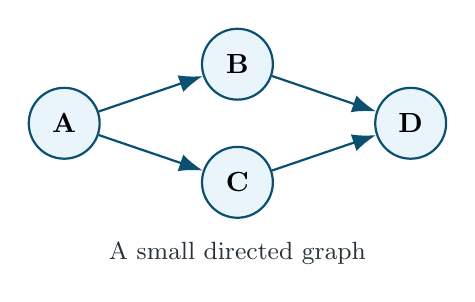
\begin{tikzpicture}[
  node/.style={circle,draw=CourseBlue,fill=LightBlue,thick,minimum size=9mm,font=\bfseries},
  edge/.style={-{Latex[length=3mm]},thick,CourseBlue}
]
\node[node] (A) at (0,0) {A};
\node[node] (B) at (2.2,0.75) {B};
\node[node] (C) at (2.2,-0.75) {C};
\node[node] (D) at (4.4,0) {D};
\draw[edge] (A) -- (B);
\draw[edge] (A) -- (C);
\draw[edge] (B) -- (D);
\draw[edge] (C) -- (D);
\node[align=center,text=DarkText,font=\small] at (2.2,-1.65) {A small directed graph};
\end{tikzpicture}
\end{column}
\end{columns}
\end{frame}

\begin{frame}{Directed Graphs and Web Links}
\begin{itemize}
  \item In an \textbf{undirected graph}, an edge has no direction.
  \item In a \textbf{directed graph}, each edge has a direction.
  \item A web link is directed: if page \(A\) links to page \(B\), it does not
  mean that page \(B\) links back to page \(A\).
\end{itemize}

\[
V = \{\text{pages}\}, \qquad E = \{\text{hyperlinks}\}
\]
\end{frame}

\begin{frame}{Neighbors, Inlinks, and Outlinks}
For a page \(p\):
\begin{itemize}
  \item \textbf{Outlinks}: pages that \(p\) links to.
  \item \textbf{Inlinks}: pages that link to \(p\).
  \item \textbf{Out-degree}: the number of outlinks from \(p\).
  \item \textbf{In-degree}: the number of inlinks into \(p\).
\end{itemize}

\[
\Gamma(p)=\{q : p \rightarrow q\}, \qquad |\Gamma(p)|=\outdeg(p)
\]

\begin{block}{Important intuition}
PageRank is not just counting inlinks. A link from a strong page contributes
more, and a page that links to many pages divides its rank among them.
\end{block}
\end{frame}

\section{PageRank Basics}

\begin{frame}{Rank and Normalization}
The PageRank score of a page \(p\), written \(\PR(p)\), represents the page's
importance in the link graph.

\vspace{0.5em}
Ranks are usually normalized:
\[
\sum_{p \in V} \PR(p)=1
\]

This lets us interpret PageRank as a probability distribution over pages.
\end{frame}

\begin{frame}{Rank Flow}
Each page distributes its current rank equally among its outlinks.

\[
\text{if } \PR(A)=0.30 \text{ and } \outdeg(A)=3,
\qquad
\text{each outlink receives } \frac{0.30}{3}=0.10
\]

\centering
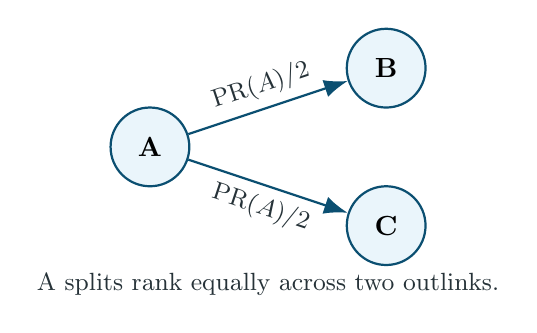
\begin{tikzpicture}[
  node/.style={circle,draw=CourseBlue,fill=LightBlue,thick,minimum size=10mm,font=\bfseries},
  flow/.style={-{Latex[length=3mm]},thick,CourseBlue},
  label/.style={font=\small,align=center,text=DarkText}
]
\node[node] (A) at (0,0) {A};
\node[node] (B) at (3,1) {B};
\node[node] (C) at (3,-1) {C};
\draw[flow] (A) -- node[label,above,sloped] {\(\PR(A)/2\)} (B);
\draw[flow] (A) -- node[label,below,sloped] {\(\PR(A)/2\)} (C);
\node[label] at (1.5,-1.75) {A splits rank equally across two outlinks.};
\end{tikzpicture}
\end{frame}

\begin{frame}{Initial Rank and Convergence}
\begin{columns}[T,onlytextwidth]
\begin{column}{0.48\textwidth}
\textbf{Initialization}
\[
\PR_0(p)=\frac{1}{N}
\]
Every page starts with equal rank.
\end{column}
\begin{column}{0.48\textwidth}
\textbf{Stopping condition}
\[
\sum_{p \in V} |\PR_{t+1}(p)-\PR_t(p)| < \varepsilon
\]
Stop when scores change only slightly.
\end{column}
\end{columns}
\end{frame}

\begin{frame}{Simple Update Rule}
Start with a directed graph where every page has at least one outlink.

\[
\PR_{t+1}(p)
=
\sum_{q \rightarrow p}
\frac{\PR_t(q)}{|\Gamma(q)|}
\]

\begin{block}{Read the formula}
The new rank of page \(p\) is the sum of all rank contributions sent by pages
that link to \(p\).
\end{block}
\end{frame}

\begin{frame}[fragile]{Simple Pseudocode}
\begin{verbatim}
initialize PR[p] = 1 / N for every page p

repeat until convergence:
    newPR[p] = 0 for every page p

    for each page q:
        contribution = PR[q] / number_of_outlinks(q)
        for each outlink p of q:
            newPR[p] += contribution

    PR = newPR
\end{verbatim}
\end{frame}

\begin{frame}{What the Algorithm Is Doing}
Each iteration has two conceptual phases:
\begin{enumerate}
  \item \textbf{Distribute}: every page sends rank mass to its out-neighbors.
  \item \textbf{Collect}: every page sums the rank mass it receives from in-neighbors.
\end{enumerate}

\begin{block}{Data-engineering view}
This is a repeated message-passing computation over graph edges.
\end{block}
\end{frame}

\section{Numerical Example}

\begin{frame}{Example Graph}
Consider three pages:
\[
V=\{A,B,C\}
\]

\[
A \rightarrow B,\qquad A \rightarrow C,\qquad B \rightarrow C,\qquad C \rightarrow A
\]

\centering
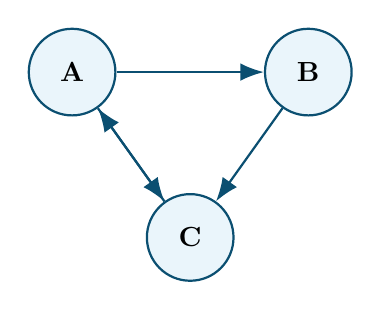
\begin{tikzpicture}[
  node/.style={circle,draw=CourseBlue,fill=LightBlue,thick,minimum size=11mm,font=\bfseries},
  edge/.style={-{Latex[length=3mm]},thick,CourseBlue}
]
\node[node] (A) at (0,1.4) {A};
\node[node] (B) at (3,1.4) {B};
\node[node] (C) at (1.5,-0.7) {C};
\draw[edge] (A) -- (B);
\draw[edge] (A) -- (C);
\draw[edge] (B) -- (C);
\draw[edge] (C) -- (A);
\end{tikzpicture}
\end{frame}

\begin{frame}{Out-Neighbor Sets}
\[
\Gamma(A)=\{B,C\}, \qquad \Gamma(B)=\{C\}, \qquad \Gamma(C)=\{A\}
\]

\[
|\Gamma(A)|=2,\qquad |\Gamma(B)|=1,\qquad |\Gamma(C)|=1
\]

\vspace{0.5em}
Initialization:
\[
\PR_0(A)=\PR_0(B)=\PR_0(C)=\frac{1}{3}
\]
\end{frame}

\begin{frame}{Iteration 1: Distribute}
Page \(A\) splits its rank between \(B\) and \(C\):
\[
A \rightarrow B: \frac{1/3}{2}=\frac{1}{6},
\qquad
A \rightarrow C: \frac{1/3}{2}=\frac{1}{6}
\]

Page \(B\) sends all its rank to \(C\):
\[
B \rightarrow C: \frac{1/3}{1}=\frac{1}{3}
\]

Page \(C\) sends all its rank to \(A\):
\[
C \rightarrow A: \frac{1/3}{1}=\frac{1}{3}
\]
\end{frame}

\begin{frame}{Iteration 1: Collect}
\[
\PR_1(A)=\frac{1}{3},
\qquad
\PR_1(B)=\frac{1}{6},
\qquad
\PR_1(C)=\frac{1}{6}+\frac{1}{3}=\frac{1}{2}
\]

\begin{center}
\small
\begin{tabular}{lccc}
\toprule
Page & \(\PR_0\) & Incoming contributions & \(\PR_1\) \\
\midrule
A & \(1/3\) & from C: \(1/3\) & \(1/3 = 0.3333\) \\
B & \(1/3\) & from A: \(1/6\) & \(1/6 = 0.1667\) \\
C & \(1/3\) & from A: \(1/6\), from B: \(1/3\) & \(1/2 = 0.5000\) \\
\bottomrule
\end{tabular}
\end{center}
\end{frame}

\begin{frame}{Iteration 2}
Use \(\PR_1(A)=1/3\), \(\PR_1(B)=1/6\), and \(\PR_1(C)=1/2\).

\[
A \rightarrow B: \frac{1}{6},
\quad
A \rightarrow C: \frac{1}{6},
\quad
B \rightarrow C: \frac{1}{6},
\quad
C \rightarrow A: \frac{1}{2}
\]

\[
\PR_2(A)=\frac{1}{2},
\qquad
\PR_2(B)=\frac{1}{6},
\qquad
\PR_2(C)=\frac{1}{3}
\]
\end{frame}

\begin{frame}{Reading the Result}
\begin{itemize}
  \item After the first iteration, page \(C\) becomes strong because both \(A\)
  and \(B\) link to it.
  \item After the second iteration, page \(A\) becomes strong because the strong
  page \(C\) links to it.
  \item The algorithm keeps moving rank through the graph until the scores
  stabilize.
\end{itemize}
\end{frame}

\section{Markov Chains}

\begin{frame}{Random Surfer Interpretation}
Imagine a user randomly surfing the web:
\begin{enumerate}
  \item The user is currently on some page.
  \item The user chooses one outgoing link uniformly at random.
  \item The user moves to the linked page.
  \item This repeats many times.
\end{enumerate}

\begin{block}{Interpretation}
The PageRank score of a page is the long-run probability that the random surfer
is on that page.
\end{block}
\end{frame}

\begin{frame}{What Is a Markov Chain?}
A Markov chain is a probabilistic process where the next state depends only on
the current state, not on the full history.

\vspace{0.5em}
For PageRank:
\begin{itemize}
  \item States are pages.
  \item Transitions are hyperlinks.
  \item Transition probabilities are usually uniform over outlinks.
\end{itemize}
\end{frame}

\begin{frame}{Transition Matrix}
For the graph \(A \rightarrow B\), \(A \rightarrow C\), \(B \rightarrow C\),
\(C \rightarrow A\):

\[
M_{ij} =
\begin{cases}
\frac{1}{\outdeg(j)} & \text{if page } j \text{ links to page } i,\\
0 & \text{otherwise}
\end{cases}
\]

\[
M =
\begin{bmatrix}
0 & 0 & 1 \\
\frac{1}{2} & 0 & 0 \\
\frac{1}{2} & 1 & 0
\end{bmatrix}
\]
\end{frame}

\begin{frame}{Matrix-Vector Update}
The PageRank update can be written as:
\[
\rankvec_{t+1}=M\rankvec_t
\]

At convergence:
\[
\rankvec = M\rankvec
\]

\begin{block}{Stationary distribution}
\(\rankvec\) is a stationary distribution of the Markov chain and an eigenvector
of \(M\) with eigenvalue \(1\).
\end{block}
\end{frame}

\begin{frame}{Bridge to Data Engineering}
PageRank has two equivalent views:
\begin{itemize}
  \item an iterative graph algorithm that sends messages along edges;
  \item repeated sparse matrix-vector multiplication.
\end{itemize}

\begin{block}{Why this matters}
Both views lead naturally to distributed implementations.
\end{block}
\end{frame}

\section{Damping}

\begin{frame}{Why the Simple Algorithm Is Not Enough}
\begin{columns}[T,onlytextwidth]
\begin{column}{0.48\textwidth}
\textbf{Dangling nodes}

A dangling node has no outlinks:
\[
D \rightarrow \varnothing
\]
Its rank disappears unless handled.
\end{column}
\begin{column}{0.48\textwidth}
\textbf{Spider traps}

A group of pages can point only to itself. Rank can get stuck permanently inside
the group.
\end{column}
\end{columns}
\end{frame}

\begin{frame}{Damping}
Damping modifies the random surfer model:
\begin{itemize}
  \item With probability \(d\), the surfer follows an outgoing link.
  \item With probability \(1-d\), the surfer teleports to a random page.
\end{itemize}

\[
d=0.85
\]

The surfer follows links \(85\%\) of the time and teleports \(15\%\) of the time.
\end{frame}

\begin{frame}{Why Damping Helps}
\begin{itemize}
  \item Prevents rank from getting stuck permanently in spider traps.
  \item Gives dangling-node rank a principled way to re-enter the graph.
  \item Makes every page reachable with positive probability.
  \item Helps guarantee a unique stable PageRank vector.
\end{itemize}
\end{frame}

\begin{frame}{Damped Update Formula}
Let \(N\) be the number of pages, \(d\) the damping factor, and \(M_t\) the total
rank mass of dangling nodes at iteration \(t\).

\[
\PR_{t+1}(p)
=
\frac{1-d}{N}
+
d \left(
\sum_{q \rightarrow p}
\frac{\PR_t(q)}{|\Gamma(q)|}
+
\frac{M_t}{N}
\right)
\]

\begin{enumerate}
  \item \(\frac{1-d}{N}\): teleportation mass.
  \item Link-based contributions from in-neighbors.
  \item \(\frac{M_t}{N}\): redistributed dangling-node mass.
\end{enumerate}
\end{frame}

\begin{frame}{Damped Example: Setup}
\[
A \rightarrow B,\quad A \rightarrow C,\quad B \rightarrow C,\quad C \rightarrow A,
\quad D \rightarrow \varnothing
\]

\[
N=4,\qquad
\PR_0(A)=\PR_0(B)=\PR_0(C)=\PR_0(D)=0.25,\qquad
d=0.85
\]

\[
M_0=\PR_0(D)=0.25,
\qquad
\frac{M_0}{N}=0.0625,
\qquad
\frac{1-d}{N}=0.0375
\]
\end{frame}

\begin{frame}{Damped Example: Iteration 1}
Incoming link contributions:
\[
\mathrm{in}(A)=0.25,\quad
\mathrm{in}(B)=0.125,\quad
\mathrm{in}(C)=0.375,\quad
\mathrm{in}(D)=0
\]

\[
\PR_1(p)=0.0375+0.85\left(\mathrm{in}(p)+0.0625\right)
\]

\begin{center}
\small
\begin{tabular}{lccc}
\toprule
Page & Link contribution & Formula & \(\PR_1\) \\
\midrule
A & 0.2500 & \(0.0375+0.85(0.3125)\) & 0.3031 \\
B & 0.1250 & \(0.0375+0.85(0.1875)\) & 0.1969 \\
C & 0.3750 & \(0.0375+0.85(0.4375)\) & 0.4094 \\
D & 0.0000 & \(0.0375+0.85(0.0625)\) & 0.0906 \\
\bottomrule
\end{tabular}
\end{center}
\end{frame}

\section{MapReduce}

\begin{frame}{PageRank as a Distributed Data Problem}
The web graph is huge:
\begin{itemize}
  \item billions of pages;
  \item many billions of links;
  \item sparse but too large for one machine;
  \item iterative computation: the graph is processed many times.
\end{itemize}

This makes PageRank a natural example for MapReduce and other distributed data
systems.
\end{frame}

\begin{frame}{Data Representation}
Each page can be represented as:
\[
(\text{page}, \text{current rank}, \text{adjacency list})
\]

\begin{center}
\begin{tabular}{lll}
\toprule
Page & Current rank & Adjacency list \\
\midrule
A & 0.25 & [B, C] \\
B & 0.25 & [C] \\
C & 0.25 & [A] \\
D & 0.25 & [] \\
\bottomrule
\end{tabular}
\end{center}
\end{frame}

\begin{frame}{One Iteration as MapReduce}
\begin{enumerate}
  \item \textbf{Map}: each page emits rank contributions to its outlinks.
  \item \textbf{Map}: each page also emits its adjacency list so the graph
  structure is preserved.
  \item \textbf{Shuffle}: contributions are grouped by destination page.
  \item \textbf{Reduce}: each page sums incoming contributions and applies damping.
  \item \textbf{Repeat}: run another iteration using the new ranks.
\end{enumerate}
\end{frame}

\begin{frame}{MapReduce Flow}
\begin{figure}
\centering
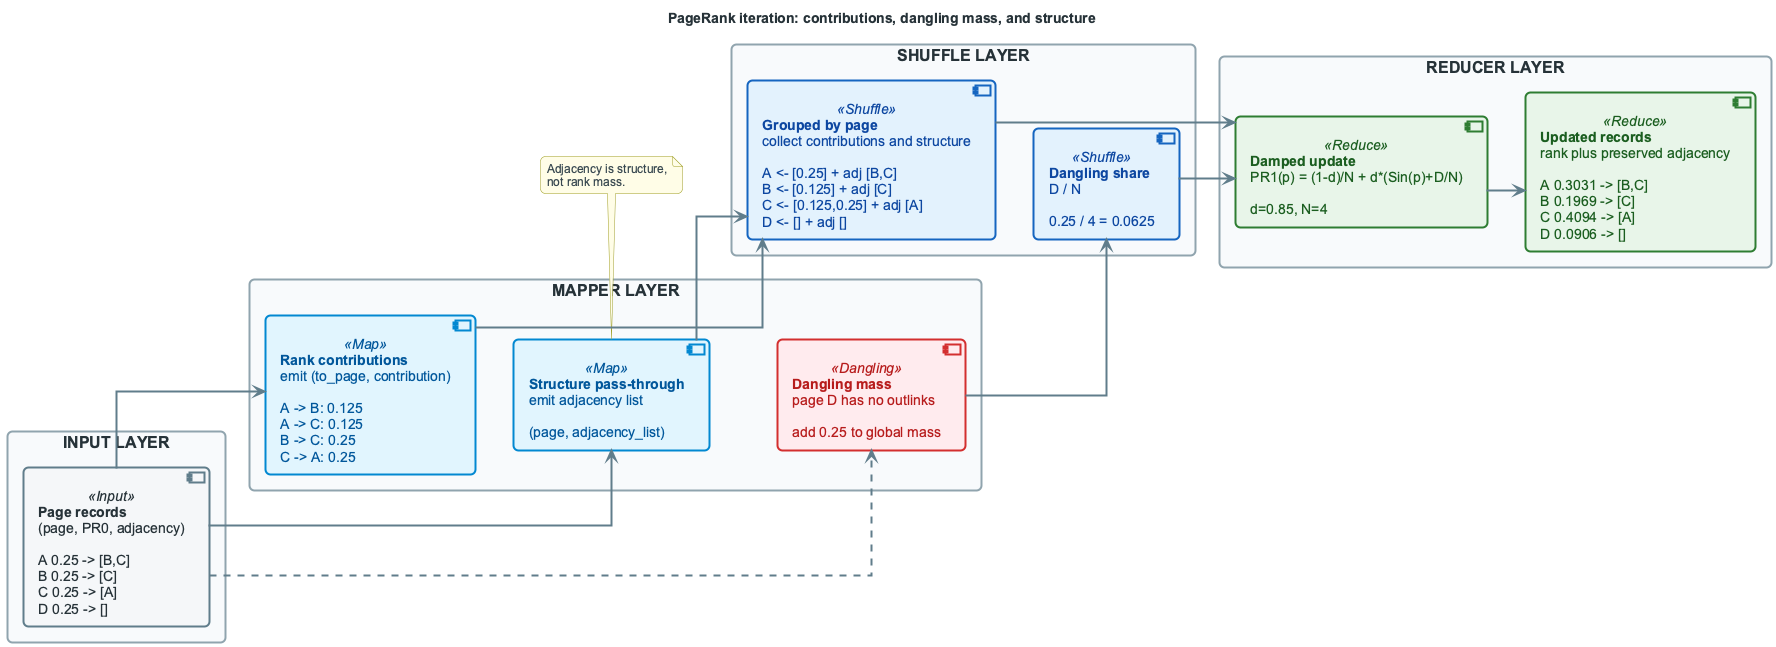
\includegraphics[width=0.92\linewidth]{week7_pagerank_iteration_flow.png}
\caption{One PageRank iteration as a MapReduce dataflow.}
\end{figure}
\end{frame}

\begin{frame}{Mapper}
Input:
\[
(p, \PR_t(p), \Gamma(p))
\]

If \(p\) has outlinks:
\[
\text{for each } q \in \Gamma(p),\quad
\mathrm{emit}(q, \PR_t(p)/|\Gamma(p)|)
\]

Also preserve graph structure:
\[
\mathrm{emit}(p, \mathrm{AdjacencyList}(\Gamma(p)))
\]

If \(p\) is dangling, add \(\PR_t(p)\) to global dangling mass.
\end{frame}

\begin{frame}{Reducer}
Input for a page \(p\):
\[
(p, [\text{values grouped by key }p])
\]

The values contain numeric contributions from in-neighbors and one adjacency list.

\[
\mathrm{sum\_in}(p)=\sum \text{numeric contributions received by }p
\]

\[
\PR_{t+1}(p)=
\frac{1-d}{N}+d\left(\mathrm{sum\_in}(p)+\frac{M_t}{N}\right)
\]

The reducer emits \((p, \PR_{t+1}(p), \Gamma(p))\).
\end{frame}

\begin{frame}[fragile]{Formal MapReduce Pseudocode}
\begin{verbatim}
map(page p, rank r, adjacency list L):
    emit(p, STRUCTURE(L))

    if L is empty:
        add r to DANGLING_MASS
    else:
        c = r / length(L)
        for each destination q in L:
            emit(q, CONTRIBUTION(c))

combine(page p, values):
    sum numeric CONTRIBUTION values
    pass STRUCTURE values unchanged
\end{verbatim}
\end{frame}

\begin{frame}[fragile]{Formal MapReduce Pseudocode: Reduce}
\begin{verbatim}
reduce(page p, values):
    L = adjacency list from STRUCTURE value
    s = sum all CONTRIBUTION values
    newRank = (1 - d) / N + d * (s + DANGLING_MASS / N)
    emit(p, newRank, L)
\end{verbatim}
\end{frame}

\begin{frame}{MapReduce Example: Input}
\begin{center}
\begin{tabular}{lll}
\toprule
Page & Rank & Outlinks \\
\midrule
A & 0.25 & [B, C] \\
B & 0.25 & [C] \\
C & 0.25 & [A] \\
D & 0.25 & [] \\
\bottomrule
\end{tabular}
\end{center}
\end{frame}

\begin{frame}{MapReduce Example: Mapper Emissions}
\begin{center}
\small
\begin{tabular}{lll}
\toprule
Source page & Emitted key & Emitted value \\
\midrule
A & B & contribution 0.125 \\
A & C & contribution 0.125 \\
A & A & structure [B, C] \\
B & C & contribution 0.250 \\
B & B & structure [C] \\
C & A & contribution 0.250 \\
C & C & structure [A] \\
D & D & structure [] \\
D & global & dangling mass 0.250 \\
\bottomrule
\end{tabular}
\end{center}
\end{frame}

\begin{frame}{MapReduce Example: Shuffle and Reduce}
\begin{columns}[T,onlytextwidth]
\begin{column}{0.53\textwidth}
\small
\textbf{After shuffle}
\resizebox{\linewidth}{!}{%
\begin{tabular}{ll}
\toprule
Key & Values \\
\midrule
A & contribution 0.250, structure [B, C] \\
B & contribution 0.125, structure [C] \\
C & contribution 0.125, contribution 0.250, structure [A] \\
D & structure [] \\
\bottomrule
\end{tabular}
}
\end{column}
\begin{column}{0.42\textwidth}
\small
\textbf{Reducer output}
\resizebox{\linewidth}{!}{%
\begin{tabular}{lll}
\toprule
Page & New rank & Structure \\
\midrule
A & 0.3031 & [B, C] \\
B & 0.1969 & [C] \\
C & 0.4094 & [A] \\
D & 0.0906 & [] \\
\bottomrule
\end{tabular}
}
\end{column}
\end{columns}
\end{frame}

\begin{frame}{Engineering Notes}
\begin{itemize}
  \item \textbf{Combiner}: safe for numeric contribution sums; must preserve adjacency lists.
  \item \textbf{Dangling mass}: track with a counter, special key, or separate aggregation job.
  \item \textbf{Convergence}: reducers can emit \(|\PR_{t+1}(p)-\PR_t(p)|\).
  \item \textbf{Cost}: each iteration scans the graph and shuffles \(O(|E|)\) data.
  \item \textbf{Skew}: hot pages may need two-stage aggregation.
\end{itemize}
\end{frame}

\section{Wrap-Up}

\begin{frame}{Summary}
\begin{itemize}
  \item A web graph is a directed graph: pages are nodes, links are edges.
  \item Basic PageRank repeatedly sends each page's rank through its outgoing links.
  \item PageRank is also a Markov chain: ranks are long-run visit probabilities.
  \item Damping adds teleportation, handles dangling nodes, and prevents rank traps.
  \item MapReduce implements each iteration as contribution emission, shuffle,
  and reduction by summation plus damping.
\end{itemize}
\end{frame}

\begin{frame}{Practice Questions}
\begin{enumerate}
  \item Given \(A\rightarrow B\), \(B\rightarrow C\), \(C\rightarrow A\), and
  \(D\rightarrow C\), compute one simple PageRank iteration from equal initialization.
  \item For the same graph, write the transition matrix \(M\).
  \item Add damping with \(d=0.85\). If there are no dangling nodes, what changes?
  \item Explain why the adjacency list must pass through mapper and reducer.
  \item Suppose one page receives \(40\%\) of all graph links. What MapReduce
  bottleneck might appear, and how could you reduce it?
\end{enumerate}
\end{frame}

\end{document}
